

{\color{gray}\hrule}
\begin{center}
\section{European Vanilla Put Option Pricing}
% \textbf{You can add small descriptions of what the current sections describe}
\bigskip
\end{center}
{\color{gray}\hrule}
\begin{multicols}{2}

\subsection{Problem Statement}
Pricing a European Vanilla Option is a key concept in financial engineering. Here, we are pricing a put option, which gives the buyer the right and not the obligation to sell an asset at a fixed price, called the strike price (\(K\)), on a future date (\(T\)). 

The payoff at maturity depends on how the asset price (\(S_T\)) compares to \(K\) and is calculated as:
\[\text{Payoff} = \max(0, K - S_T)
\]
If the asset price falls below the strike price, the option has value; otherwise, it expires worthless. 

The theoretical price of this option is calculated using the Black-Scholes-Merton model, which considers the expected value of the payoff, adjusted for the time value of money:
$$
    p = e^{-rT} \mathbb{E}[\max(0, K - S_T)]
$$
Here:
\begin{itemize}
    \item \(r\): the risk-free interest rate, which accounts for continuous compounding.
    \item \(K\): the strike price of the option.
    \item \(S_T\): the asset price at maturity.
\end{itemize}

In this project, our goal is to estimate the price of the option using Monte Carlo simulations, which use random sampling to approximate the expected value. We'll also explore how increasing the number of simulations (\(N\)) improves accuracy. 

The results will include:
\begin{itemize}
    \item Estimated option price.
    \item Error margins and confidence intervals (CI).
    \item Computation time.
    \item Difference from the exact Black-Scholes price.
\end{itemize}

\subsection{Methodology}

For N simulations, we create a new instance of the \texttt{Option} class. Each instance initializes values according to the Problem setup discussed further. The stock price is simulated using random numbers generated using the normal distribution. Based on these prices at t=T, the payoff is calculated, discounted and returned for that particular price path. We then take the arithmetic average across all such N paths which gives the final value for the option.

The sample mean $(\mathbb{E}[P])$ and the mean of the square of price $(\mathbb{E}[{P^2})$ which gives the standard error,

$$
    se(Payoff) = \sqrt{\frac{\mathbb{E}[{P^2}] - (\mathbb{E}[P])^2}{N - 1}}
$$

We can construct the 100(1-$\alpha$)\% confidence interval using the Central limit theorem and the above standard error for the estimate.

\subsubsection{Problem Setup}

We aim to price an European Put option using Monte Carlo simulations under the following setup:

\begin{itemize}
    \item Spot price $(S_o) = \$100$
    \item Strike price $K = \$100 $
    \item Time to Maturity $(T)$ = 0.5 year
    \item Risk-free Rate $(r) = 4\%$
    \item Dividend yield $(q) = 2\%$
    \item Volatility $(\sigma) = 20\%$
\end{itemize}

The convergence of the Monte Carlo method is evaluated by varying the number of simulated paths (N) and analyzing the results. We vary N by a factor of 4. This is in line with the theoretical convergence of $1/\sqrt{n}$ for Monte Carlo. By varying by a factor of 4, we aim to observe a reduction in standard error by \textbf{half}.

\subsubsection{Variance Reduction Technique: Antithetic Approach\cite{POUDEL}}

The Antithetic variate approach uses a synthetic asset which is perfectly negatively correlated with the original asset. The synthetic asset is called the antithetic variate. Consider the assets,

$dS_{1,t} = rS_{1,t}dt + \sigma S_{1,t}dZ_t$

$dS_{1,t} = rS_{1,t}dt - \sigma S_{1,t}dZ_t$

The r, $\sigma$, time to maturity are all the same and the starting price is also the same. Thus, the analytical value of the option for both these paths will be the same. If the two options were combined, we would observe $var(0.5(S_1+S_2)) < var(S_1)$ and $var(0.5(S_1+S_2)) < var(S_2)$\cite{POUDEL}. This is because the assets are negatively correlated. Any movement results in  negative co-movement and thus the resulting payoff observes very less movement.

We then have the following payoffs for our put option,
$$
    P_{T} = (K - S(0) exp(\sqrt{T}+\sigma \sqrt{T}(Z))^+
$$
$$
    P_{T}^* = (K - S(0)exp(\sqrt{T}+\sigma \sqrt{T}(-Z))^+
$$
where, $Z \thicksim \mathcal{N}(0,1)$. In our simulation, we can then take the mean of these two payoffs and assign it as our final payoff for the put option.

%Richardson Extrapolation is used to enhance the accuracy of Monte Carlo simulation results by reducing the bias associated with discretization. The approach involves:
%\begin{itemize}
%   \item Running simulations at two different levels of granularity.
%    \item Combining results to cancel out leading-order error terms.
%\end{itemize}
%Imagine you're trying to measure something, but your tools aren’t perfect—they give you slightly different results depending on how precise you try to be. Richardson Extrapolation helps you combine those results to cancel out the main errors and get a better answer.
\subsection{Results}
The following table(Table 1) summarizes the results of the Monte Carlo simulation, showing the option price, estimated standard error (SE), 95\% confidence interval, absolute pricing error, and computation time for different sample sizes (\(N\)).

\subsubsection{Convergence Analysis}
\textbf{Option Price and Absolute Error:}  
European Option price estimate for the selected parameters with an accuracy upto a cent is \textbf{\$5.07}. 

As the sample size increased, the estimated option price steadily converged toward the true value. At \(N = 256,000\), the absolute pricing error was minimal at just 0.002222, demonstrating a highly accurate estimate. Beyond this sample size, further increases provided only marginal improvements in accuracy, indicating diminishing returns.


\textbf{Estimated Standard Error (SE):}  
The standard error decreased with larger sample sizes, reflecting greater precision in the estimates. For \(N = 4,096,000\), the SE was as low as 0.00354899, highlighting the reliability of the simulation at higher sample sizes. 

We can clearly observe that the standard error is halved every time the number of simulations is increased by 4, which is in line with the $\frac{1}{\sqrt{n}}$ convergence of Monte Carlo.

\textbf{Confidence Intervals:}  
The 95\% confidence intervals narrowed significantly as the sample size grew, offering greater certainty in the estimated price. For \(N = 4,096,000\), the interval was \([5.06534, 5.07925]\), indicating a high degree of confidence in the results.

\end{multicols}
\begin{table}[h!]
\centering
\caption{Summary of Results}
\begin{tabular}{|p{1.8cm}|p{1.8cm}|p{2cm}|p{4cm}|p{2cm}|p{2cm}|}
\hline
\textbf{Sample Size (\(N\))} & \textbf{Option Price} & \textbf{Estimated SE} & \textbf{95\% C.I.} & \textbf{Absolute Pricing Error} & \textbf{Compute Time (s)} \\ \hline
1,000      & 5.62406  & 0.24316   & [5.14747, 6.10064] & 0.549421  & 0.001396 \\ \hline
4,000      & 5.32484  & 0.115344  & [5.09877, 5.55091] & 0.250203  & 0.004458 \\ \hline
16,000     & 5.13141  & 0.0568855 & [5.01992, 5.2429]  & 0.056773  & 0.017990 \\ \hline
64,000     & 5.0646   & 0.0283004 & [5.00913, 5.12007] & 0.010036  & 0.074846 \\ \hline
256,000    & 5.07241  & 0.0142032 & [5.04458, 5.10025] & 0.002222  & 0.228177 \\ \hline
1,024,000  & 5.08877  & 0.00711048 & [5.07483, 5.10271] & 0.014134  & 0.875244 \\ \hline
4,096,000  & 5.07229  & 0.00354899 & [5.06534, 5.07925] & 0.002343  & 3.53752  \\ \hline
20,000,000  & 5.07678  & 0.00177545 & [5.0733, 5.08026] & 0.002147  & 17.457s  \\ \hline
\end{tabular}
\end{table}
\begin{figure}
    \centering
    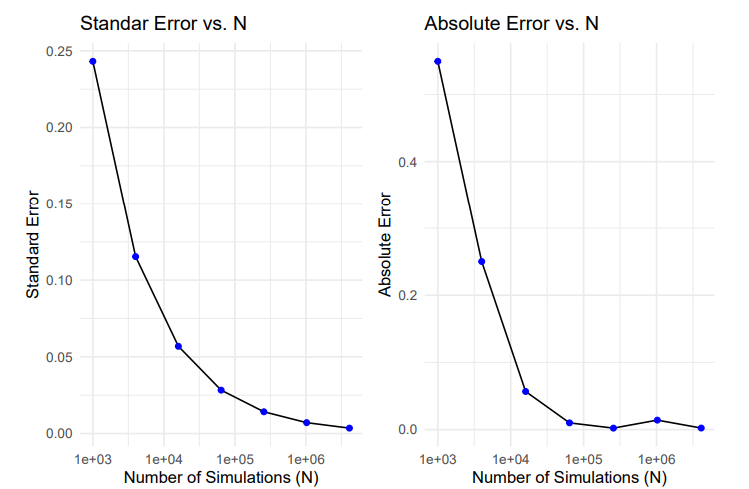
\includegraphics[width=0.8\linewidth]{1.png}
    \caption{Error - Simulations}
    \label{fig:enter-label}
\end{figure}
\begin{multicols}{2}
\subsubsection{Computational Performance}
\textbf{Computation Time:}  
The computation time increased proportionally with the sample size. For \(N = 1,000\), the simulation completed in just 0.001396 seconds, whereas for \(N = 4,096,000\), it required 3.53752 seconds, reflecting the tradeoff between precision and computational demand.

\textbf{Efficiency-Accuracy Tradeoff:}  
While larger sample sizes improved accuracy and precision, they also demanded significantly more computational resources. For practical purposes, \(N = 256,000\) strikes a good balance between accuracy and efficiency, delivering results with minimal error and reasonable computation time.

\subsubsection{Antithetic Approach}
The antithetic variates approach is used in Monte Carlo simulations to make option pricing more accurate and efficient. Instead of using random samples, it creates pairs of related samples that are negatively correlated. For example, if a random movement in the underlying asset price is generated, an opposite movement is also created by using the opposite signs for the random numbers. By averaging the results of these paired paths, the approach reduces random fluctuations and provides a more stable estimate of the option price. 
\end{multicols}
\begin{table}[h!]
\centering
\caption{Antithetic Method Results}
\vspace{4pt}
\begin{tabular}{|p{1.8cm}|p{1.8cm}|p{2cm}|p{4cm}|p{2cm}|p{2cm}|}
\hline
\textbf{Sample Size (\(N\))} & \textbf{Option Price} & \textbf{Estimated SE} & \textbf{95\% Confidence Interval} & \textbf{Absolute Pricing Error} & \textbf{Compute Time (s)} \\ \hline
256,000    & 5.07394  & 0.00710851 & [5.06001, 5.08787] & 0.000698  & 0.196551 \\ \hline
20,000,000  & 5.07427  & 0.000888735 & [5.07253, 5.07602] & 0.000362  & 16.9786  \\ \hline
\end{tabular}
\end{table}
\begin{figure}
    \centering
    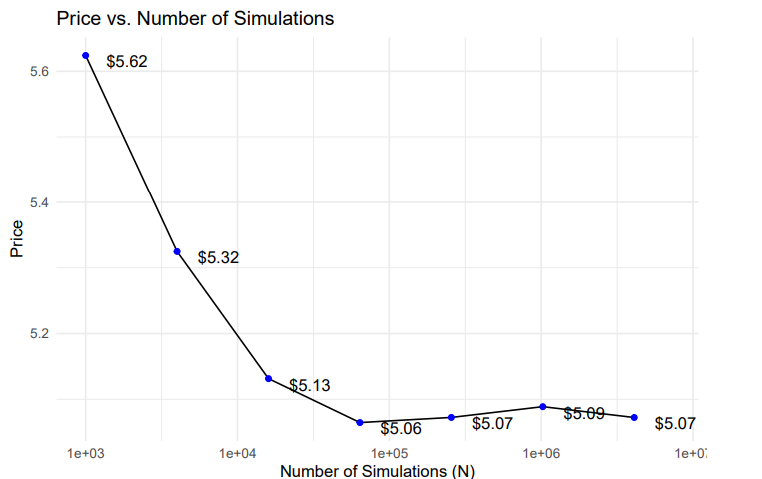
\includegraphics[width=0.8\linewidth]{2.png}
    \caption{Price - Simulations}
    \label{fig:enter-label}
\end{figure}
\begin{multicols}{2}
\textbf{Improved Accuracy:}  
For the optimal sample size of \(N = 256,000\):
\begin{itemize}
    \item \textbf{Standard Monte Carlo:} Option price = 5.07241 with an absolute pricing error of 0.002222.
    \item \textbf{Antithetic Method:} Option price = 5.07394 with an absolute pricing error of 0.000698.
\end{itemize}
The antithetic approach significantly reduces the absolute error while maintaining the same number of samples.

\textbf{Lower Standard Error:}  
The Estimated Standard Error (SE) is consistently lower using the antithetic method:
\begin{itemize}
    \item For \(N = 256,000\), SE = 0.00710851 in the antithetic method versus 0.0142032 in the standard method.
    \item For \(N = 20,000,000\), SE reduces further to 0.000887758 in the antithetic method.
\end{itemize}
This demonstrates that the antithetic variates technique achieves higher precision with reduced variance.

\textbf{Narrower Confidence Intervals:}  
The 95\% confidence intervals are narrower with the antithetic method, indicating greater certainty in the estimates.

\textbf{Comparable or Better Computational Efficiency:}  
While the computation time increases slightly with larger \(N\), the antithetic method achieves a more accurate and precise result. For example:
\begin{itemize}
    \item For \(N = 20,000,000\), the antithetic method required 16.9786 seconds, whereas the standard Monte Carlo took 17.457 seconds.
\end{itemize}

In summary, the antithetic variates approach not only improves accuracy and precision but also demonstrates computational efficiency, making it a superior choice for pricing options using Monte Carlo methods.
\subsection{Discussion}

The results of the Monte Carlo simulations for pricing the European vanilla put option demonstrate the impact of sample size and variance reduction techniques, particularly the antithetic variates approach, on accuracy, precision, and computational efficiency.
\subsubsection{Comparison of Methods}

The comparison between the standard Monte Carlo method and the antithetic variates approach clearly highlights the advantages of the latter. The absolute pricing error using the antithetic method was reduced compared to the standard method. The antithetic method consistently produced a smaller standard error and the 95\% confidence intervals were significantly narrower indicating greater certainty in the option price estimate.
\subsubsection{Convergence Behavior}
The results validate the theoretical convergence rate of \(1/\sqrt{N}\) for Monte Carlo simulations. As the sample size \(N\) increased, the option price approached the true value, and the standard error decreased proportionally. However, the effect diminished for very large \(N\) where increases in sample size gave us marginal improvements in accuracy and required significantly more compute time.  Additionally, in comparison to the standard Monte Carlo method, the antithetic method achieved more accurate results in slightly less time (e.g., 16.9786s for \(N = 20,000,000\)).
\end{multicols}
\begin{figure}
    \centering
    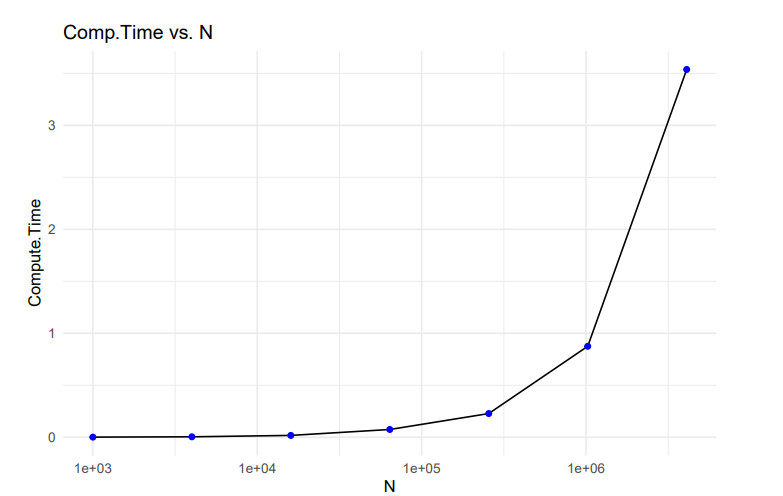
\includegraphics[width=0.8\linewidth]{3.png}
    \caption{Computation Time - Simulations}
    \label{fig:enter-label}
\end{figure}
\begin{figure}
    \centering
    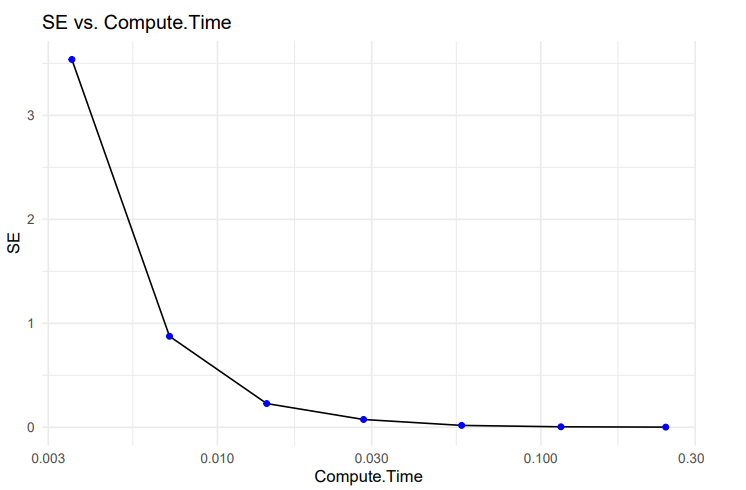
\includegraphics[width=0.8\linewidth]{4.png}
    \caption{Computation Time - Standard Error}
    \label{fig:enter-label}
\end{figure}
\begin{multicols}{2}
This highlights the efficiency-accuracy tradeoff: the antithetic variates approach delivers better results with minimal additional computational cost, making it particularly valuable for time-sensitive applications.
\subsubsection*{Practical Implications of Variance Reduction}
The antithetic method proves to be a powerful variance reduction technique for Monte Carlo simulations. By generating negatively correlated movements and averaging their payoffs, the method reduces random fluctuations, improves accuracy, and decreases standard error without requiring a significant increase in the sample size.

In real-world applications, such as financial risk management or high frequency trading, where computational resources are limited, the antithetic approach can provide faster, more reliable option pricing results.
\subsubsection*{Limitations and Future Work}
While the antithetic method significantly improves accuracy and precision, it may not be sufficient for options with more complex payoffs, such as path-dependent options or American options. Future work can explore combining antithetic variates with other variance reduction techniques, such as control variates or stratified sampling, to achieve even better results. Additionally, leveraging parallel computing could help reduce computational time for very large \(N\).
\subsubsection{Key Insights}
\begin{itemize}
    \item The antithetic variates method reduces variance and improves the accuracy of Monte Carlo simulations without an increase in the computation time.
    \item For practical purposes, a sample size of \(N = 256,000\) strikes an effective balance between accuracy and efficiency.
    \item The method’s ability to produce narrower confidence intervals and lower standard errors makes it a valuable enhancement for option pricing models.
\end{itemize}

\end{multicols}
